\chapter{Design patterns}

\section{Model View Controller}

\subsection{MVC Description}
The MVC is implemented by using JavaFX. If you look at the figure below, you see the principle of the MVC design pattern. The model is loaded by creating a Stage with a FXML file as resource. The Stage is the View for the user and the FXML file also creates a designated controller (MainController, StartController and GameEndController). The View properties can be loaded using @FXML tags. Now, when the user interacts, the information is sent to the designated controller that in turn sents the information to the View. 

In reality, it's more like the figure below.
\\
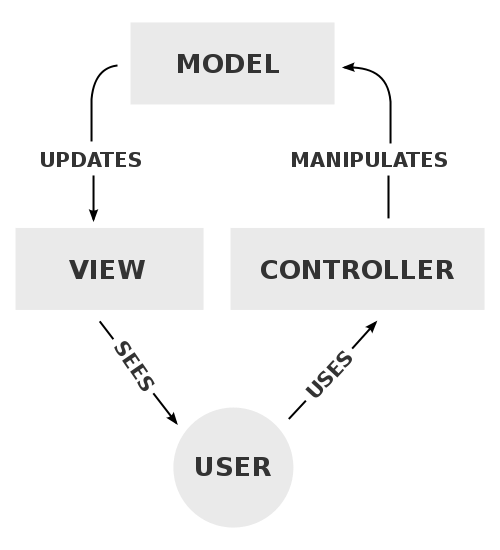
\includegraphics[width=100mm]{MVC.png}

\subsection{MVC Class Diagram}

Below is the class diagram of the Model View Controller design pattern, found in our code.
\\
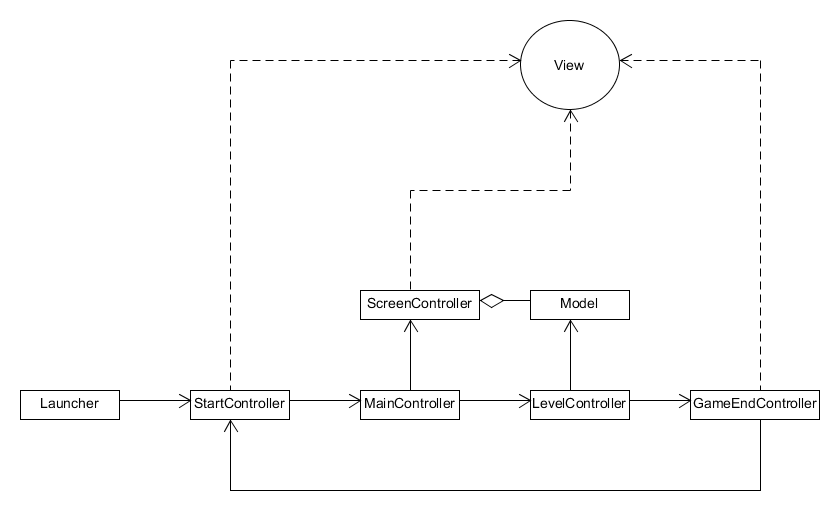
\includegraphics[width=100mm]{UML_MVC.png}

\subsection{MVC Sequence Diagram}
`Make a sequence diagram of how the pattern works dynamically in your code'